\documentclass[aspectratio=169]{beamer}\usepackage[]{graphicx}\usepackage[]{color}
% maxwidth is the original width if it is less than linewidth
% otherwise use linewidth (to make sure the graphics do not exceed the margin)
\makeatletter
\def\maxwidth{ %
  \ifdim\Gin@nat@width>\linewidth
    \linewidth
  \else
    \Gin@nat@width
  \fi
}
\makeatother

\definecolor{fgcolor}{rgb}{0.345, 0.345, 0.345}
\newcommand{\hlnum}[1]{\textcolor[rgb]{0.686,0.059,0.569}{#1}}%
\newcommand{\hlstr}[1]{\textcolor[rgb]{0.192,0.494,0.8}{#1}}%
\newcommand{\hlcom}[1]{\textcolor[rgb]{0.678,0.584,0.686}{\textit{#1}}}%
\newcommand{\hlopt}[1]{\textcolor[rgb]{0,0,0}{#1}}%
\newcommand{\hlstd}[1]{\textcolor[rgb]{0.345,0.345,0.345}{#1}}%
\newcommand{\hlkwa}[1]{\textcolor[rgb]{0.161,0.373,0.58}{\textbf{#1}}}%
\newcommand{\hlkwb}[1]{\textcolor[rgb]{0.69,0.353,0.396}{#1}}%
\newcommand{\hlkwc}[1]{\textcolor[rgb]{0.333,0.667,0.333}{#1}}%
\newcommand{\hlkwd}[1]{\textcolor[rgb]{0.737,0.353,0.396}{\textbf{#1}}}%
\let\hlipl\hlkwb

\usepackage{framed}
\makeatletter
\newenvironment{kframe}{%
 \def\at@end@of@kframe{}%
 \ifinner\ifhmode%
  \def\at@end@of@kframe{\end{minipage}}%
  \begin{minipage}{\columnwidth}%
 \fi\fi%
 \def\FrameCommand##1{\hskip\@totalleftmargin \hskip-\fboxsep
 \colorbox{shadecolor}{##1}\hskip-\fboxsep
     % There is no \\@totalrightmargin, so:
     \hskip-\linewidth \hskip-\@totalleftmargin \hskip\columnwidth}%
 \MakeFramed {\advance\hsize-\width
   \@totalleftmargin\z@ \linewidth\hsize
   \@setminipage}}%
 {\par\unskip\endMakeFramed%
 \at@end@of@kframe}
\makeatother

\definecolor{shadecolor}{rgb}{.97, .97, .97}
\definecolor{messagecolor}{rgb}{0, 0, 0}
\definecolor{warningcolor}{rgb}{1, 0, 1}
\definecolor{errorcolor}{rgb}{1, 0, 0}
\newenvironment{knitrout}{}{} % an empty environment to be redefined in TeX

\usepackage{alltt}
\usepackage{multirow}
%\usecolortheme{beaver}
%\usecolortheme[RGB={129,3,3}]{structure}
\usetheme{CambridgeUS}
\usecolortheme{seahorse}

% Standard header (will need to change date!)
\title[GEOG 5680 Summer '20]{GEOG 5680\\Introduction to R}
\subtitle[Intro]{07: Plotting with \textbf{ggplot2}}
\author[S. Brewer]{Simon Brewer}
\institute[Univ. Utah]{
  Geography Department\\
  University of Utah\\
  Salt Lake City, Utah 84112\\[1ex]
  \texttt{simon.brewer@geog.utah.edu}
}
\date[May 03, 2020]{May 03, 2020}
\IfFileExists{upquote.sty}{\usepackage{upquote}}{}
\begin{document}


%--- the titlepage frame -------------------------%
\begin{frame}
  \titlepage
\end{frame}

% %--- Slide 3 ----------------%
% \begin{frame}{Objectives}
% \begin{itemize}
%   \item Introduce \textbf{ggplot2}
%   \item Dataframes for \textbf{ggplot2}
%   \item Examples
% \end{itemize}
% \end{frame}

\section{ggplot2}
%--- Slide 3 ----------------%
\begin{frame}{ggplot2}
\begin{columns}
  \begin{column}{0.6\textwidth}
\begin{itemize}
  \item Based on Leland Wilkinson's Grammar of Graphics
  \begin{itemize}
    \item All data figures can be represented by the same \emph{grammar}
  \end{itemize}
  \item Adapted for R by Hadley Wickham
  \item Provides much easier methods for comparative plots
\end{itemize}
  \end{column}
  \begin{column}{0.4\textwidth}
  \begin{center}
      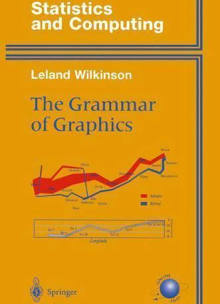
\includegraphics[width=0.65\textwidth]{./images/wilkinson.png}
  \end{center}
  \end{column}
\end{columns}
\end{frame}

%--- Slide 3 ----------------%
\begin{frame}[fragile]{Base graphics vs. ggplot2}
\begin{columns}
  \begin{column}{0.50\textwidth}
  Base graphics: 8 lines
\begin{knitrout}\scriptsize
\definecolor{shadecolor}{rgb}{0.969, 0.969, 0.969}\color{fgcolor}
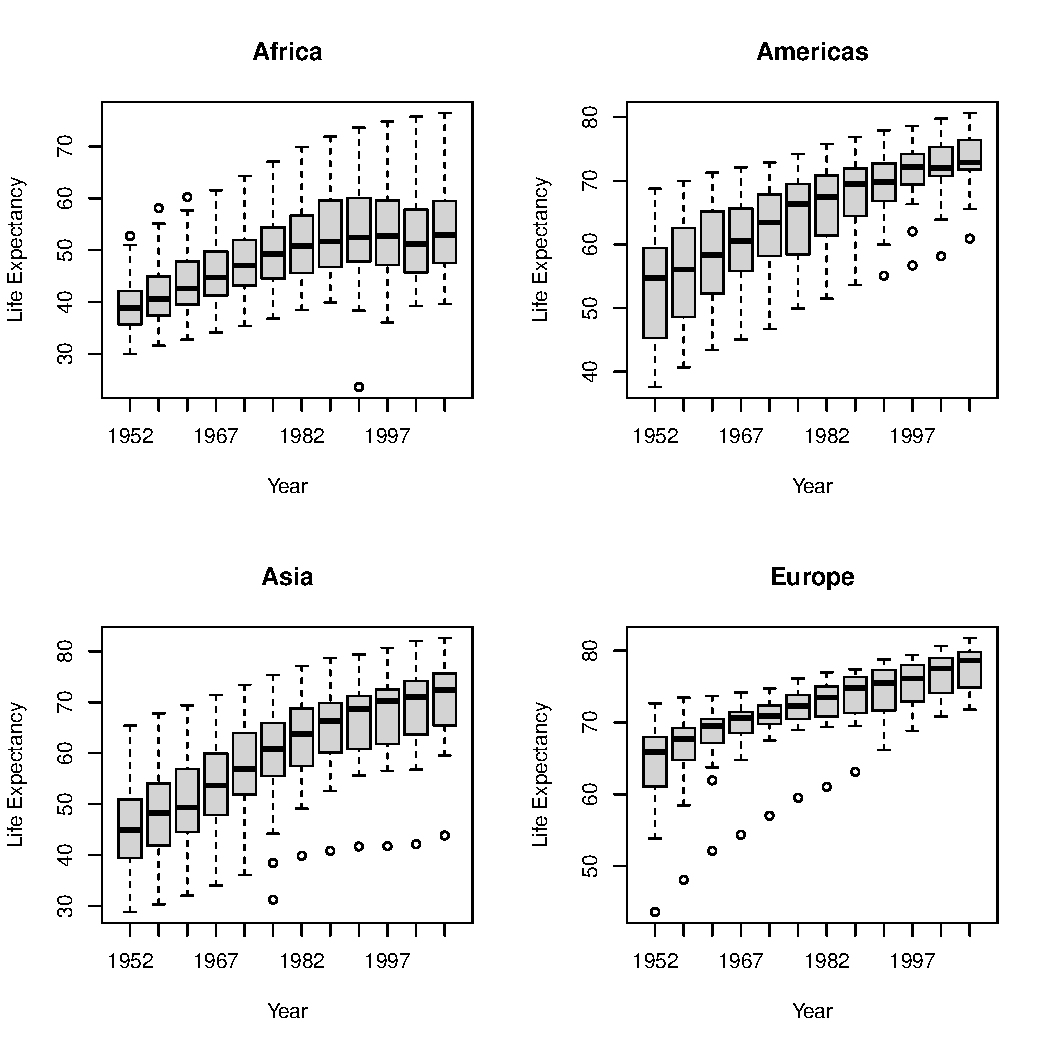
\includegraphics[width=\maxwidth]{figure/unnamed-chunk-1-1} 

\end{knitrout}
  \end{column}
  \begin{column}{0.5\textwidth}
  ggplot2: 1 (quite complex) line
\begin{knitrout}\scriptsize
\definecolor{shadecolor}{rgb}{0.969, 0.969, 0.969}\color{fgcolor}
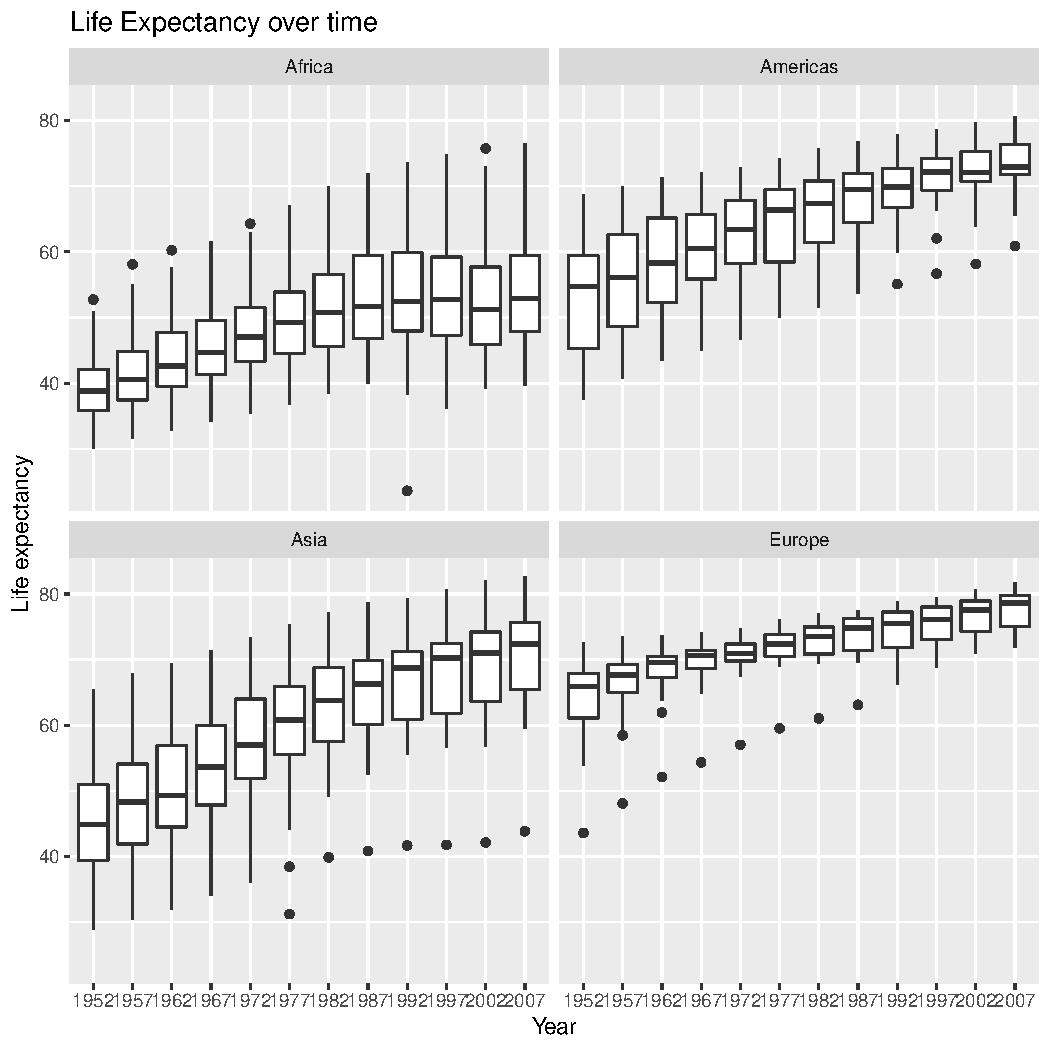
\includegraphics[width=\maxwidth]{figure/unnamed-chunk-2-1} 

\end{knitrout}
  \end{column}
\end{columns}
\end{frame}

\section{Data frames for ggplot2}
\begin{frame}[fragile]{Data frames for ggplot2}
\begin{columns}
  \begin{column}{0.50\textwidth}
    \begin{itemize}
      \item Data is often presented as short and fat tables
      \item Plotting is easier with tall and thin data frames
      \begin{itemize}
        \item Each variable forms a column
        \item Each observation forms a row
      \end{itemize}
    \end{itemize}
  \end{column}
	\begin{column}{0.5\textwidth}
  \begin{center}
      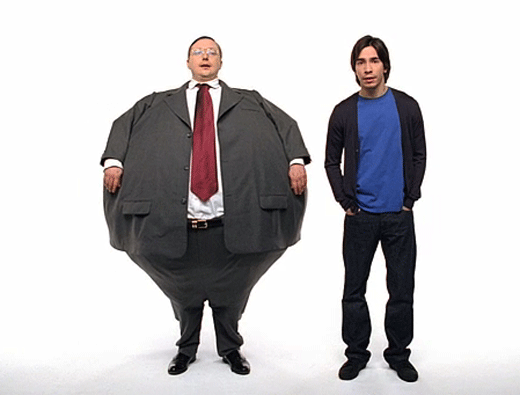
\includegraphics[width=0.95\textwidth]{./images/fat_vs_thin.png}
  \end{center}
  \end{column}
\end{columns}
\end{frame}

\begin{frame}[fragile]{Data frames for ggplot2}
%\Fontvi
\begin{columns}
  \begin{column}{0.50\textwidth}
Short/fat table: good for presenting results
\begin{tabular}{ l | c r }
  \hline
   & TreatA & TreatB \\
  \hline 
  Jane Smith & - & 2 \\
  John Doe & 16 & 11 \\
  Mary Jones & 3 & 1 \\
  \hline
\end{tabular}
\end{column}
  \begin{column}{0.5\textwidth}
Tall/thin dataframe: preferred for plotting
\begin{tabular}{ l | c | r }
  \hline 
  Name & Treat & Result \\
  \hline 
  Jane Smith & a & - \\
  John Doe & a & 16 \\
  Mary Jones & a & 3 \\
  Jane Smith & b & 2 \\
  John Doe & b & 11 \\
  Mary Jones & b & 1 \\
  \hline 
\end{tabular}

\end{column}
\end{columns}
\begin{itemize}
  \item Support package \textbf{reshape2} includes functions to transform between these layouts
  \item \texttt{cast}: thin data frame to table
  \item \texttt{melt}: table to thin data frame 
\end{itemize}
\end{frame}

\section{Grammar of Graphics}
\begin{frame}{Grammar of Graphics}
\begin{columns}
  \begin{column}{0.5\textwidth}
  \begin{itemize}
    \item Theme: font, colors, etc
    \item Coordinates: plotting space
    \item Statistics: summaries/transformation of data
    \item Facet: subplots based on groups
    \item Geometry: shapes used to represent data
    \item Aesthetic: scale used to map data
    \item Data: as data frame
  \end{itemize}
  \end{column}
  \begin{column}{0.5\textwidth}
  \begin{center}
      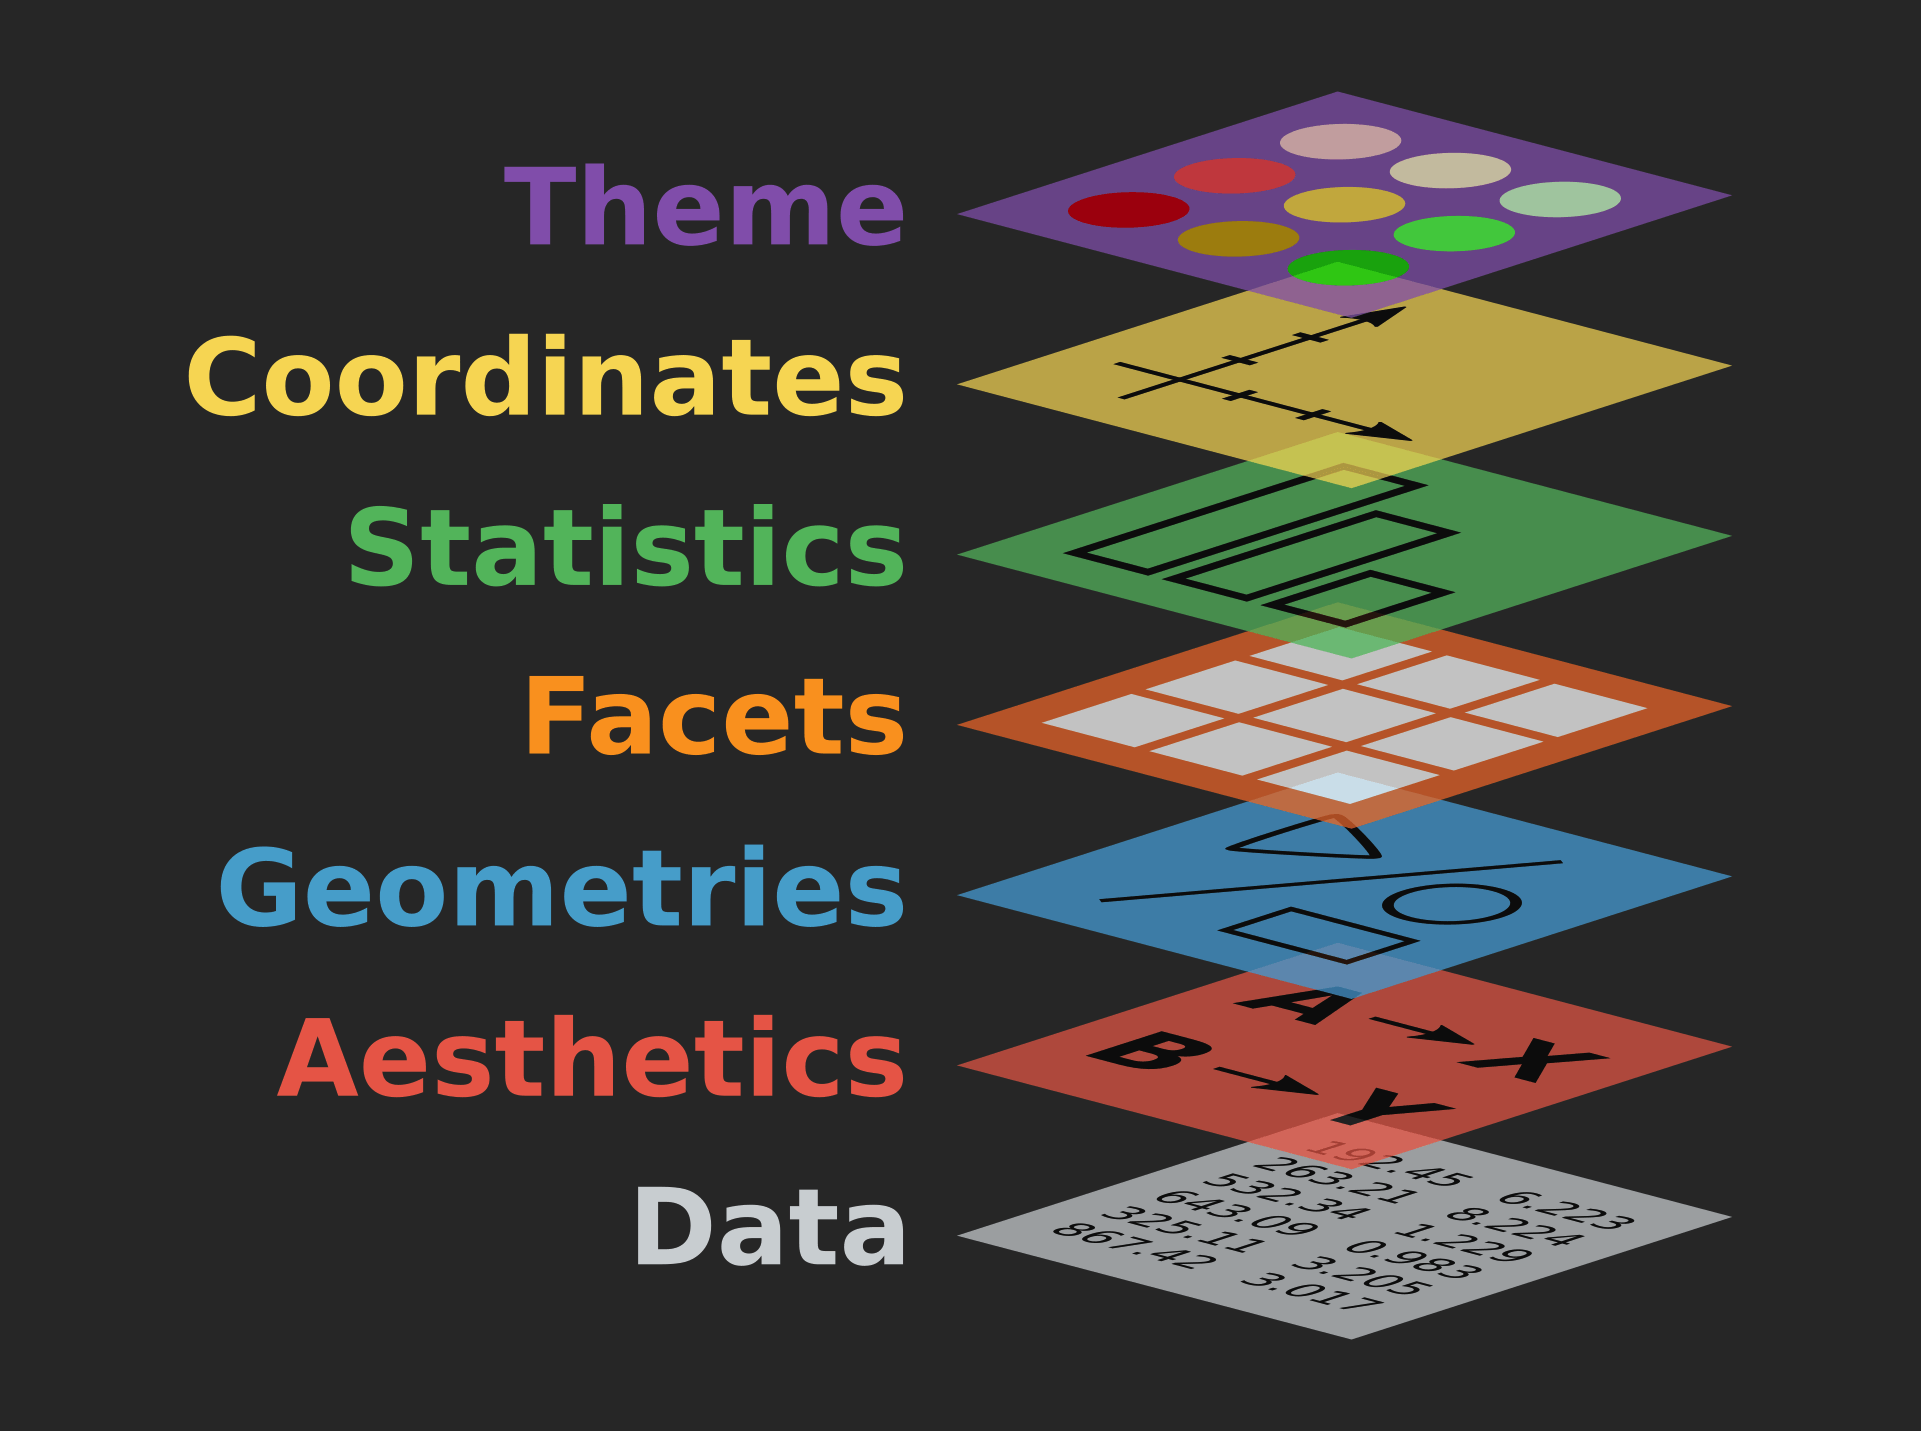
\includegraphics[width=0.85\textwidth]{./images/gglayers.png}
  \end{center}
  \end{column}
\end{columns}
\end{frame}

% \section{Examples}
% \begin{frame}[fragile]{Simple scatterplot}
% <<echo=FALSE>>=
% data(iris) 
% @
% <<fig.height=4>>=
% myplot = ggplot(data=iris, aes(x=Sepal.Length, y=Petal.Length)) 
% myplot + geom_point()
% @
% \end{frame}
% 
% \begin{frame}[fragile]{Simple scatterplot}
% <<fig.height=4>>=
% myplot = ggplot(data=iris, aes(x=Sepal.Length, y=Petal.Length,
%                                color=Species)) 
% myplot + geom_point()
% @
% \end{frame}
% 
% \begin{frame}[fragile]{Smoothing lines}
% <<fig.height=4, message=FALSE>>=
% myplot = ggplot(data=iris, aes(x=Sepal.Length, y=Petal.Length,
%                                color=Species)) 
% myplot + geom_point() + geom_smooth()
% @
% \end{frame}
% 
% \begin{frame}[fragile]{Themes}
% <<echo=FALSE, message=FALSE>>=
% require(ggthemes)
% myplot = ggplot(data=iris, aes(x=Sepal.Length, y=Petal.Length,
%                                color=Species)) 
% @
% <<fig.height=4, message=FALSE>>=
% myplot + geom_point() + geom_smooth() + 
%   ggtitle("Fisher's Iris Dataset") + theme_bw()
% @
% \end{frame}
% 
% \begin{frame}[fragile]{Themes}
% <<fig.height=4, message=FALSE>>=
% myplot + geom_point() + geom_smooth() + 
%   ggtitle("Fisher's Iris Dataset") + theme_economist()
% @
% \end{frame}
% 
% \begin{frame}[fragile]{Histogram}
% <<fig.height=4, message=FALSE>>=
% myplot = ggplot(data=iris, aes(x=Sepal.Length, fill=Species))
% myplot + geom_histogram(binwidth = 0.1)
% @
% \end{frame}
% 
% \begin{frame}[fragile]{Boxplot}
% <<fig.height=4>>=
% myplot = ggplot(data=iris, aes(x=Species, y=Sepal.Length))
% myplot + geom_boxplot()
% @
% \end{frame}
% 
% \begin{frame}[fragile]{Scales}
% <<fig.height=4>>=
% myplot = ggplot(data=gapdata, aes(x=gdpPercap, y=lifeExp))
% myplot + geom_point()
% @
% \end{frame}
% 
% \begin{frame}[fragile]{Scales}
% <<fig.height=4>>=
% myplot = ggplot(data=gapdata, aes(x=gdpPercap, y=lifeExp))
% myplot + geom_point() + scale_x_log10()
% @
% \end{frame}
% 
% \begin{frame}[fragile]{Facets}
% <<fig.height=4>>=
% myplot = ggplot(data=gapdata, aes(x=gdpPercap, y=lifeExp))
% myplot + geom_point() + scale_x_log10() + facet_wrap(~continent)
% @
% \end{frame}
% 
% \begin{frame}[fragile]{Facets}
% <<fig.height=4>>=
% myplot = ggplot(data=subset(gapdata, continent != "Oceania"), 
%                 aes(x=gdpPercap, y=lifeExp))
% myplot + geom_point() + scale_x_log10() + facet_grid(year~continent)
% @
% \end{frame}
% 
% \begin{frame}[fragile]{Facets}
% <<fig.height=4>>=
% myplot + geom_point() + scale_x_log10() + 
%   facet_grid(year~continent) + geom_smooth(method = "lm")
% @
% \end{frame}
% 
% \begin{frame}[fragile]{ggmap}
% \begin{columns}
% \begin{column}{0.5\textwidth}
%   Google Maps API
% <<echo=FALSE, message=FALSE>>=
% library(ggmap)
% map = get_map(location="Mont Blanc France", zoom=12, 
%               source="google", maptype="terrain")
% ggmap(map)
% @
% \end{column}
% \begin{column}{0.5\textwidth}
%   Stamen Maps API
% <<echo=FALSE, message=FALSE>>=
% map = get_map(location="Ponte Vecchio Florence", zoom=17, 
%               source="stamen", maptype="toner")
% ggmap(map)
% @
% \end{column}
% \end{columns}
% \end{frame}
% 
% %--- Slide ----------------%
% \begin{frame}{Next Class}
% \begin{itemize}
%   \item Lab: Plotting with \textbf{ggplot2}
% 	\item 0402: Statistical models in R
% \end{itemize}
% \end{frame}

\end{document}
